% Figure snippets for embedding in main.tex (schematic + data-grounded).

\begin{figure}[htbp]
\centering
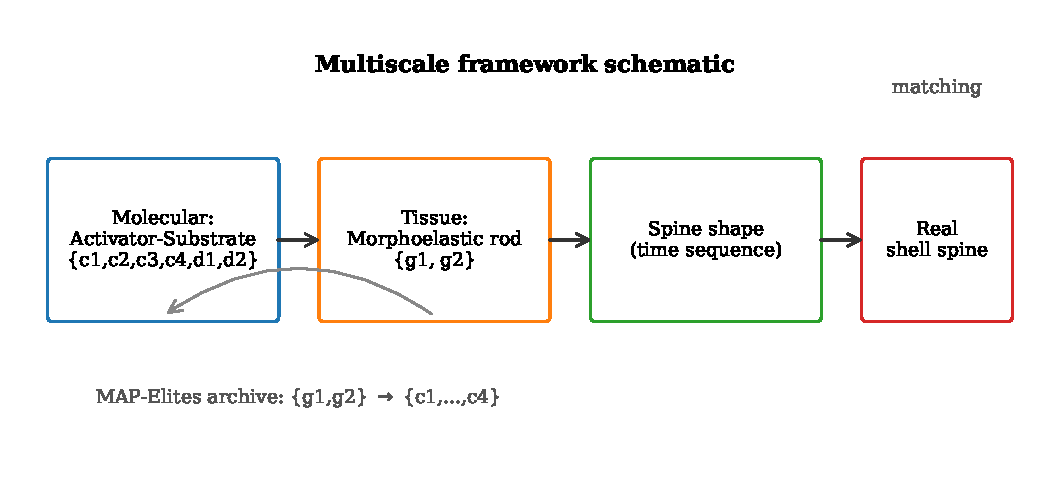
\includegraphics[width=0.95\textwidth]{figures/fig_framework.pdf}
\caption{Schematic of the multiscale framework. A molecular Activator-Substrate
reaction-diffusion model with parameters $\{c_1,c_2,c_3,c_4,d_1,d_2\}$
generates a spatial concentration profile that is mapped to the parameters
$\{g_1, g_2\}$ of a Gaussian growth profile at the tissue scale. The
morphoelastic rod model then evolves a spine shape which is compared against
real shell images. A MAP-Elites archive connects the tissue-scale
$\{g_1, g_2\}$ space back to molecular parameter sets.}
\label{fig:framework}
\end{figure}

\begin{figure}[htbp]
\centering
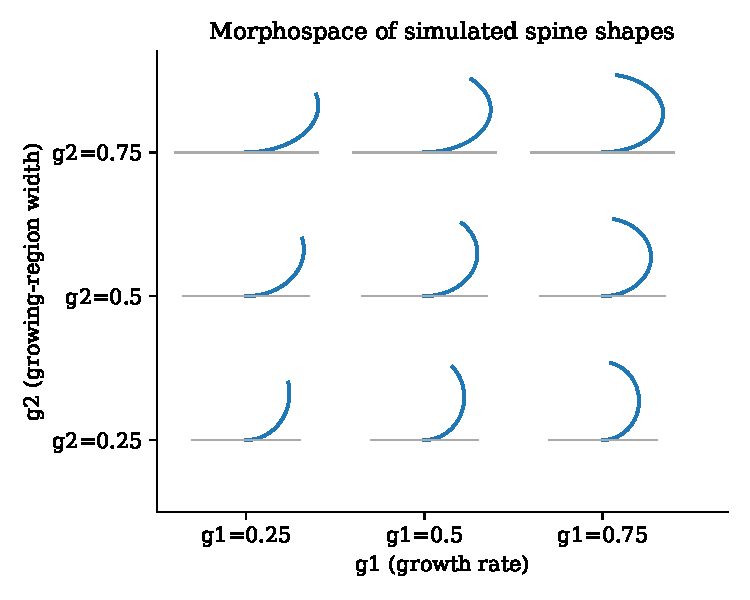
\includegraphics[width=0.65\textwidth]{figures/fig_morphospace.pdf}
\caption{Qualitative morphospace of simulated spine shapes as the Gaussian
growth parameters $g_1$ (rate) and $g_2$ (width) are varied. Larger $g_1$
produces more curved spines that reach self-contact earlier, while larger
$g_2$ produces wider spines. Schematic only; the axes illustrate the
structural trend described in the text.}
\label{fig:morphospace}
\end{figure}

\begin{figure}[htbp]
\centering
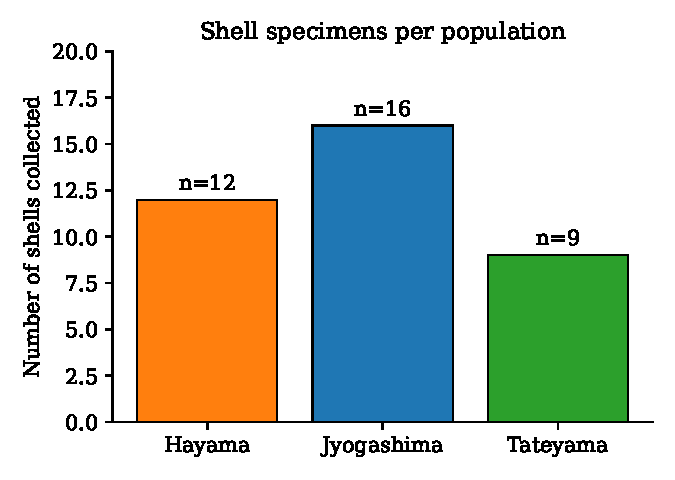
\includegraphics[width=0.6\textwidth]{figures/fig_sample_sizes.pdf}
\caption{Sample sizes of \textit{Turbo sazae} shell specimens collected at
each of the three Japanese localities: $n=12$ from Hayama, $n=16$ from
Jyogashima, and $n=9$ from Tateyama.}
\label{fig:samples}
\end{figure}

\begin{figure}[htbp]
\centering
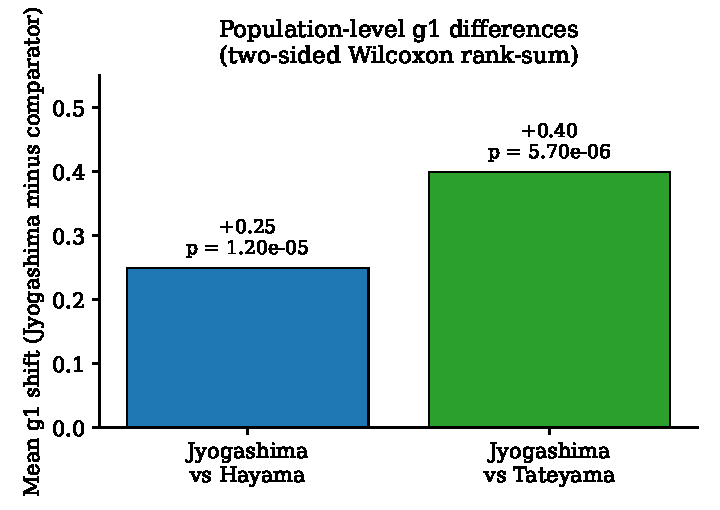
\includegraphics[width=0.7\textwidth]{figures/fig_population_g1.pdf}
\caption{Population-level differences in the tissue-scale growth parameter
$g_1$. Two-sided Wilcoxon rank-sum tests show that $g_1$ values for the
Jyogashima population are on average $0.25$ higher than those from Hayama
($p = 1.202 \times 10^{-5}$) and $0.4$ higher than those from Tateyama
($p = 5.7 \times 10^{-6}$). Hayama and Tateyama do not differ significantly.}
\label{fig:g1shift}
\end{figure}
